%%%%%%%%%%%%%%%%%%%%%%%%%%%%%%%%%%%%%%%%%%%%%%%%%%%%%%%%%%%%%%%%%%%%%%%%%%%%%%%%
%%%%%%%%%%%%%%%%%%%%%%%%%%%%%%%%%%%%%%%%%%%%%%%%%%%%%%%%%%%%%%%%%%%%%%%%%%%%%%%%
%
% A general frame for lecture slides and lecture notes in one file
% using LaTeX beamer
%
%%%%%%%%%%%%%%%%%%%%%%%%%%%%%%%%%%%%%%%%%%%%%%%%%%%%%%%%%%%%%%%%%%%%%%%%%%%%%%%%
%%%%%%%%%%%%%%%%%%%%%%%%%%%%%%%%%%%%%%%%%%%%%%%%%%%%%%%%%%%%%%%%%%%%%%%%%%%%%%%%
\documentclass[ignorenonframetext,11pt]{beamer}
%\usepackage[ngerman]{babel}
%\usepackage[T1]{fontenc}
\usepackage[utf8]{inputenc}
\usepackage{lmodern}
\usepackage{amsmath,amssymb,amsfonts}


% only presentation
\mode<presentation>
{
  \usetheme{default}
%  \usecolortheme{crane}
  \setbeamercovered{transparent}
%  \setlength{\parindent}{0pt}
%  \setlength{\parskip}{1.35ex plus 0.5ex minus 0.3ex}
%  \usefonttheme{structuresmallcapsserif}
  \usefonttheme{structurebold}
  \setbeamertemplate{theorems}[numbered]
  \usepackage{amscd}
}

% all after
\usepackage{tikz}
\usepackage{pgfplots,adjustbox}
\usepackage{eurosym}
\usepackage{graphicx}
\usepackage{multimedia}
\usepackage{psfrag}
\usepackage{listings}
\lstset{language=C++, basicstyle=\ttfamily,
  keywordstyle=\color{black}\bfseries, tabsize=4, stringstyle=\ttfamily,
  commentstyle=\it, extendedchars=true, escapeinside={/*@}{@*/}}
\usepackage{curves}
%\usepackage{epic}
\usepackage{calc}
%\usepackage{picinpar}
%\usepackage{fancybox}
%\usepackage{xspace}
\usepackage{enumerate}
\usepackage{algpseudocode}
\usepackage{color}
\usepackage{bold-extra}
\usepackage{bm}
\usepackage{stmaryrd}
%\usepackage[squaren]{SIunits}
\usepackage{nicefrac}

\usepackage{fancyvrb,bbm,xspace}
\usepackage{lmodern}
\usepackage{fancyvrb,bbm,xspace}
\usepackage[binary-units]{siunitx}
\usepackage{xcolor,tabu}

\definecolor{niceblue}{rgb}{0.122,0.396,0.651}   %% 31, 101, 166 or #1F65A6
\definecolor{niceorange}{RGB}{255,205,86}        %% #FFCD56
\definecolor{nicered}{RGB}{220,20,60}                      %% rgb(220, 20, 60)
\definecolor{niceteal}{HTML}{00A9AB}
\definecolor{niceviolet}{HTML}{820080}

\definecolor{niceblueLight}{HTML}{91CAFB}
\definecolor{niceblueVeryLight}{HTML}{DDEFFF}

\usepackage{dsfont}

%\newcommand{\hlineabove}{\rule{0pt}{2.6ex}}
%\newcommand{\hlinebelow}{\rule[-1.2ex]{0pt}{0pt}}

%\usecolortheme[RGB={37,75,123}]{structure}
% \definecolor{structurecolor}{rgb}{0.905,0.318,0.071}

% \setbeamercolor{frametitle}{fg=black,bg=}
% \setbeamercolor{sidebar left}{fg=,bg=}

% \setbeamertemplate{headline}{\vskip4em}
% \setbeamersize{sidebar width left=.9cm}

% \setbeamertemplate{navigation symbols}{}
%\setbeamertemplate{blocks}[rounded][shadow=true]
%\setbeamertemplate{itemize items}[square]

\mode<presentation>
{
\theoremstyle{definition}
}
\newtheorem{Def}{Definition}%[section]
\newtheorem{Exm}[Def]{Example}
\newtheorem{Lem}[Def]{Lemma}
\newtheorem{Rem}[Def]{Remark}
\newtheorem{Rul}[Def]{Rule}
\newtheorem{Thm}[Def]{Theorem}
\newtheorem{Cor}[Def]{Corollary}
\newtheorem{Obs}[Def]{Observation}
\newtheorem{Ass}[Def]{Assumption}
\newtheorem{Pro}[Def]{Property}
\newtheorem{Alg}[Def]{Algorithm}
\newtheorem{Prp}[Def]{Proposition}
\newtheorem{Lst}[Def]{Listing}

% Delete this, if you do not want the table of contents to pop up at
% the beginning of each subsection:
\AtBeginSection[]
{
  \begin{frame}<beamer>
    \frametitle{Contents}
    \tableofcontents[sectionstyle=show/shaded,subsectionstyle=hide/hide/hide]
%\tableofcontents[currentsection]
  \end{frame}
}

% Title definition
\mode<presentation>
{
  \title{DUNE PDELab Tutorial 00\\
  {\small  An Introduction to the Finite Element Method}}
  \author{Peter Bastian}
  \institute[]
  {
   Interdisziplinäres Zentrum für Wissenschaftliches Rechnen\\
   Im Neuenheimer Feld 205, D-69120 Heidelberg \\[6pt]
  }
  \date[\today]{\today}
}


% logo nach oben
\mode<presentation>
{
% No navigation symbols and no lower logo
\setbeamertemplate{sidebar right}{}

% logo
\newsavebox{\logobox}
\sbox{\logobox}{%
    \hskip\paperwidth%
    \rlap{%
      % putting the logo should not change the vertical possition
      \vbox to 0pt{%
        \vskip-\paperheight%
        \vskip0.35cm%
        \llap{\insertlogo\hskip0.1cm}%
        % avoid overfull \vbox messages
        \vss%
      }%
    }%
}

\addtobeamertemplate{footline}{}{%
    \usebox{\logobox}%
}
}

%%%%%%%%%%%%%%%%%%%%%%%%%%%%%%%%%%%%%%%%%%%%%%%%%%%%%%%%%%%%%%%%%%%%%%%%%%%%%%%%
%%%%%%%%%%%%%%%%%%%%%%%%%%%%%%%%%%%%%%%%%%%%%%%%%%%%%%%%%%%%%%%%%%%%%%%%%%%%%%%%
%
% now comes the individual stuff lecture by lecture
%
%%%%%%%%%%%%%%%%%%%%%%%%%%%%%%%%%%%%%%%%%%%%%%%%%%%%%%%%%%%%%%%%%%%%%%%%%%%%%%%%
%%%%%%%%%%%%%%%%%%%%%%%%%%%%%%%%%%%%%%%%%%%%%%%%%%%%%%%%%%%%%%%%%%%%%%%%%%%%%%%%

\begin{document}

\frame{\titlepage}

%%%%%%%%%%%%%%%%%%%%%%%%%%%%%%%%%%%%%%%%%%%%%%%%%%%%%%%%%%%%%%%%%%%%%%%%%%%%%%%%
%%%%%%%%%%%%%%%%%%%%%%%%%%%%%%%%%%%%%%%%%%%%%%%%%%%%%%%%%%%%%%%%%%%%%%%%%%%%%%%%

\begin{frame}
\frametitle{Motivation}
\begin{itemize}
\item Start with an introduction to the finite element method (FEM) for solving Poisson's equation
with piecewise linear ``P$_1$'' finite elements
\item ``Hello World!'' for any numerical partial differential equation (PDE) solver framework!
\item Gives necessary background for \lstinline{dune-grid} module
\item Implement the method in PDELab (Wednesday)
\end{itemize}
\end{frame}

\begin{frame}
\frametitle{Challenges for PDE Software}
\begin{itemize}
\item \textbf{Many different PDE applications}
\begin{itemize}
\item Multi-physics
\item Multi-scale
\item Inverse modeling: parameter estimation, optimal control
\item Uncertainty quantification
\end{itemize}
\item \textbf{Many different numerical solution methods}
\begin{itemize}
\item No single method to solve all equations!
\item Different mesh types,  mesh generation, mesh refinement
\item Higher-order approximations (polynomial degree)
\item Error control and adaptive mesh/degree refinement
\item Iterative solution of (non-)linear algebraic equations
\end{itemize}
\item \textbf{High-performance Computing}
\begin{itemize}
\item Single core performance: Often bandwidth limited
\item Parallelization through domain decomposition
\item Robustness w.r.t. to mesh size, model parameters,  processors
\item Dynamic load balancing
\end{itemize}
\end{itemize}
$\Rightarrow$ \textbf{One software to do it all!}
\end{frame}

\begin{frame}
\frametitle{Flexibility Requires Abstraction!}
\begin{itemize}
\item DUNE/PDELab is based on an abstract formulation of the numerical scheme
based on \textbf{residual forms}
\item In order to implement a scheme it requires to put it to that form!
\item Although you might be familiar with the FEM, you might not
be familiar to the notation used here
\item When you have mastered the abstraction you can solve complex problems with
reasonable effort
\item Important feature: Orthogonality of concepts:
\begin{itemize}
\item Dimension $d=1,2,3,\ldots$
\item Linear and nonlinear
\item Stationary and Instationary
\item Scalar PDE and systems of PDEs
\item Uniform and adaptive mesh refinement of different types
\item Sequential and parallel
\end{itemize}
All that will be handled in the course!
\end{itemize}
\end{frame}

\begin{frame}
\begin{center}
\Large\textbf{Introduction to the Finite Element Method}
\end{center}
\end{frame}

%%%%%%%%%%%%%%%%%%%%%%%%%%%%%%%%%%%%%%%%%%%%%%%%%%%%%%%%%%%%%%%%%%%%%%%%%%%%%%%%
%%%%%%%%%%%%%%%%%%%%%%%%%%%%%%%%%%%%%%%%%%%%%%%%%%%%%%%%%%%%%%%%%%%%%%%%%%%%%%%%

\begin{frame}
\frametitle{Strong Formulation of the PDE Problem}
We solve Poisson's equation with inhomogeneous Dirichlet boundary conditions:
\begin{subequations}
\begin{align}
-\Delta u & = f \qquad\text{in $\Omega$},\label{eq:1a}\\
u &= g \qquad\text{on $\partial\Omega$},\label{eq:1b}
\end{align}
\end{subequations}
\begin{itemize}
\item $\Omega\subset\mathbb{R}^d$ is a polygonal domain in $d$-dimensional space
\item A function $u\in C^2(\Omega)\cap C^0(\overline\Omega)$ solving \eqref{eq:1a}, \eqref{eq:1b}
is called {\em strong solution}
\item Inhomogeneous Dirichlet boundary conditions could be
reduced to {\em homogeneous} ones: we will not do this!
\item Proving existence and uniqueness of solutions of strong solutions
requires quite restrictive conditions on $f$ and $g$
\end{itemize}
\end{frame}

\begin{frame}
\frametitle{Weak Formulation of the PDE Problem}

Suppose $u$ is a strong solution and take  {\em any test function}
$v\in C^1(\Omega)\cap C^0(\overline\Omega)$ with $v=0$ on $\partial\Omega$ then:
\begin{equation*}
\int_\Omega (-\Delta u) v \,dx =
\underbrace{\int_\Omega \nabla u \cdot \nabla v \,dx}_{=: a(u,v)}=
\underbrace{\int_\Omega fv \,dx}_{=: l(v)}.
\end{equation*}
{\em Question}:  Is there a vector space of functions $V$ with $V_g=\{v\in V :
\text{$v=g$ on $\partial\Omega$}\}$ and $V_0=\{v\in V :
\text{$v=0$ on $\partial\Omega$}\}$ such that
the problem
\begin{equation}
u \in V_g :\qquad a(u,v) = l(v) \qquad \forall v\in V_0 \label{eq:weakform}
\end{equation}
has a unique solution?

{\em Answer}: Yes, $V=H^1(\Omega)$. This $u$ is called {\em weak solution}.

Advantage: Weak solutions do exist under less restrictive conditions on the data.
\end{frame}

\begin{frame}
\frametitle{The Finite Element Method}
\begin{itemize}
\item The finite element method (FEM) is one method for the numerical solution of
PDEs
\item Others are the finite volume method (FVM) or the finite difference method (FDM)
\item The FEM is based on the weak formulation derived above
\item Its basic idea is to replace the space $V$ by a {\em finite-dimensional space} $V_h$!
\item The construction of these finite-dimensional spaces
needs some preparations \ldots
\end{itemize}
\end{frame}

\begin{frame}
\frametitle{Finite Element Mesh}
\vspace{-5mm}
\begin{center}\small
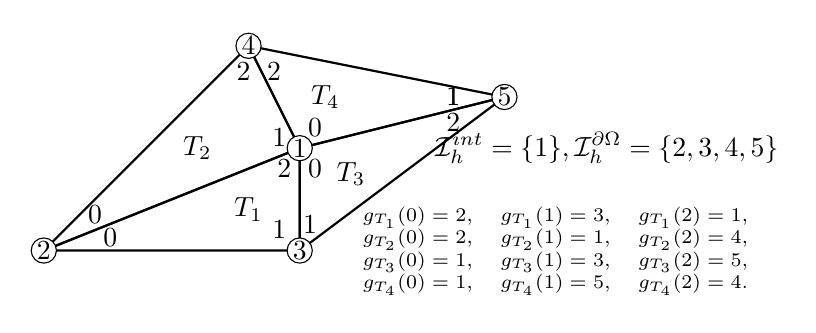
\begin{tikzpicture}[scale=0.65,baseline=(current bounding box.center)]
\draw[thick] (0,0) -- (5,0) -- (5,2) -- cycle;
\draw[thick] (0,0) -- (5,2) -- (4,4) -- cycle;
\draw[thick] (5,0) -- (9,3) -- (5,2) -- cycle;
\draw[thick] (5,2) -- (9,3) -- (4,4) -- cycle;
\node at (4,0.8) {$T_1$};
\node at (3,2) {$T_2$};
\node at (6,1.5) {$T_3$};
\node at (5.5,3) {$T_4$};
\filldraw[fill=white,draw=black] (5,2) circle (7pt) node {$1$};
\filldraw[fill=white,draw=black] (0,0) circle (7pt) node {$2$};
\filldraw[fill=white,draw=black] (5,0) circle (7pt) node {$3$};
\filldraw[fill=white,draw=black] (4,4) circle (7pt) node {$4$};
\filldraw[fill=white,draw=black] (9,3) circle (7pt) node {$5$};
\node at (1.3,0.25) {$0$}; % 2
\node at (1,0.7) {$0$};
\node at (4.6,0.4) {$1$};
\node at (5.2,0.5) {$1$};
\node at (4.7,1.6) {$2$};
\node at (5.3,1.6) {$0$};
\node at (5.3,2.4) {$0$};
\node at (4.6,2.2) {$1$};
\node at (8,2.5) {$2$};
\node at (8,3) {$1$};
\node at (8,3) {$1$};
\node at (3.9,3.5) {$2$};
\node at (4.5,3.5) {$2$};
\node at (10,0) {$%
\scriptsize
\begin{array}{lll}
g_{T_1}(0) = 2, & g_{T_1}(1) = 3, & g_{T_1}(2) = 1, \\
g_{T_2}(0) = 2, & g_{T_2}(1) = 1, & g_{T_2}(2) = 4, \\
g_{T_3}(0) = 1, & g_{T_3}(1) = 3, & g_{T_3}(2) = 5, \\
g_{T_4}(0) = 1, & g_{T_4}(1) = 5, & g_{T_4}(2) = 4.
\end{array}$};
\node at (11,2) {$\mathcal{I}_h^{int}=\{1\}, \mathcal{I}_h^{\partial\Omega}=\{2,3,4,5\}$};
\end{tikzpicture}
\end{center}
\vspace{-3mm}
\begin{itemize}
\item A mesh consists of ordered sets of vertices and elements:
\begin{equation*}
\mathcal{X}_h = \{x_1,\ldots,x_N\} \subset \mathbb{R}^d, \quad
\mathcal{T}_h = \{T_1, \ldots, T_M\}
\end{equation*}
\item {\em Simplicial element}: $T=\text{convex\_hull}(x_{T,0},\ldots,x_{T,d})$
\item {\em Conforming}: Intersection is subentity
\item {\em Local to global map} : $g_T : \{0,\ldots,d\}\to\mathcal{N}$
\begin{equation*}
\forall T\in\mathcal{T}_h, 0\leq i \leq d: g_T(i) = j \Leftrightarrow x_{T,i} = x_{j} .
\end{equation*}
\item {\em Interior and boundary vertex index sets}:
$\mathcal{I}_h = \mathcal{I}_h^{int}\cup\mathcal{I}_h^{\partial\Omega}$,\\
$\mathcal{I}_h^{int} = \{i\in \mathcal{I}_h\,:\, x_i\in\Omega\},
\mathcal{I}_h^{\partial\Omega} = \{i\in \mathcal{I}_h\,:\, x_i\in\partial\Omega\}$
\end{itemize}
\end{frame}

\begin{frame}
\frametitle{Reference Element and Element Transformation}
\begin{center}
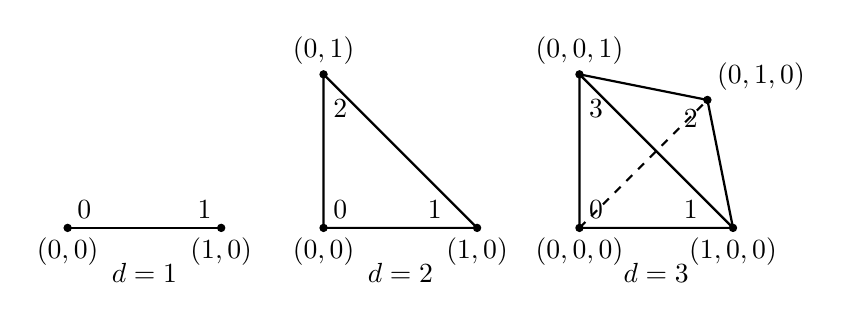
\begin{tikzpicture}[scale=0.65,baseline=(current bounding box.center)]
%d=1
\node[below] at (1.5,-0.5) {$d=1$};
\filldraw (0,0) circle [radius=2pt] node[below] {$(0,0)$}
              (3,0) circle [radius=2pt] node[below] {$(1,0)$};
\draw[thick] (0,0) -- (3,0);
\node[above right] at (0,0) {$0$};
\node[above left] at (3,0) {$1$};
%d=2
\node[below] at (6.5,-0.5) {$d=2$};
\filldraw (5,0) circle [radius=2pt] node[below] {$(0,0)$}
              (8,0) circle [radius=2pt] node[below] {$(1,0)$}
              (5,3) circle [radius=2pt] node[above] {$(0,1)$};
\draw[thick] (5,0) -- (8,0) -- (5,3) -- cycle;
\node[above right] at (5,0) {$0$};
\node[above left] at (7.5,0) {$1$};
\node[below right] at (5,2.7) {$2$};
%d=3
\node[below] at (11.5,-0.5) {$d=3$};
\filldraw (10,0) circle [radius=2pt] node[below] {$(0,0,0)$}
              (13,0) circle [radius=2pt] node[below] {$(1,0,0)$}
              (10,3) circle [radius=2pt] node[above] {$(0,0,1)$}
              (12.5,2.5) circle [radius=2pt] node[above right] {$(0,1,0)$};
\draw[thick] (10,0) -- (13,0) -- (10,3) -- cycle;
\draw[thick] (13,0) -- (12.5,2.5) -- (10,3) -- cycle;
\draw[thick,dashed] (10,0) -- (12.5,2.5);
\node[above right] at (10,0) {$0$};
\node[above left] at (12.5,0) {$1$};
\node[below left] at (12.5,2.5) {$2$};
\node[below right] at (10,2.7) {$3$};
\end{tikzpicture}
\end{center}
\begin{itemize}
\item $\hat T^d$ is the reference simplex in $d$ space dimensions
\item The mesh $\mathcal{T}_h$ is called {\em affine} if for every
$T\in\mathcal{T}_h$ there is an affine linear map $\mu_T : \hat T \to T$,
\begin{equation*}
\mu_T(\hat x) = B_T \hat x + a_T
\end{equation*}
with
$$\forall i\in\{0,\ldots,d\} : \mu_T(\hat x_i) = x_{T,i}$$
\end{itemize}
\end{frame}

\begin{frame}
\frametitle{Piecewise Linear Finite Element Space}
\begin{itemize}
\item The idea of the {\em conforming} FEM is to solve the weak problem
in {\em finite-dimensional} function spaces:
\begin{equation*}
u_h\in V_{h,g} : \quad a(u_h,v) = l(v) \quad \forall v\in V_{h,0} .
\end{equation*}
\item A particular choice is the space of {\em piecewise linear} functions
\begin{equation*}
V_h(\mathcal{T}_h) = \{ v\in C^0(\overline{\Omega}) \,:\,
\forall T\in\mathcal{T}_h : v|_T\in\mathbb{P}_1^d\}
\end{equation*}
where $\mathbb{P}_1^d = \{ p : \mathbb{R}^d \to \mathbb{R}
\,:\, p(x) = a^Tx+ b, a\in\mathbb{R}^d, b\in\mathbb{R}\}$
\item One can show $\text{dim} V_h = N = \text{dim} \mathcal{X}_h$ and $V_h\subset H^1(\Omega)$
\item {\em Lagrange} basis functions:
$$\Phi_h=\{\phi_1,\ldots,\phi_N\}, \quad
\forall i,j\in\mathcal{I}_h \,:\, \phi_i(x_j) = \delta_{i,j}$$
\item {\em Test and Ansatz spaces}:
\begin{align*}
V_{h,0} &= \{v\in V_h \,:\, \forall i\in\mathcal{I}_h^{\partial\Omega} : v(x_i)=0\}, \\
V_{h,g} &= \{v\in V_h : \forall i\in\mathcal{I}_h^{\partial\Omega} : v(x_i)=g(x_i)\} = v_{h,g} + V_{h,0}
\end{align*}
\end{itemize}
\end{frame}

\begin{frame}
\frametitle{Examples of Finite Element Functions}
Here in two space dimensions:
\begin{center}
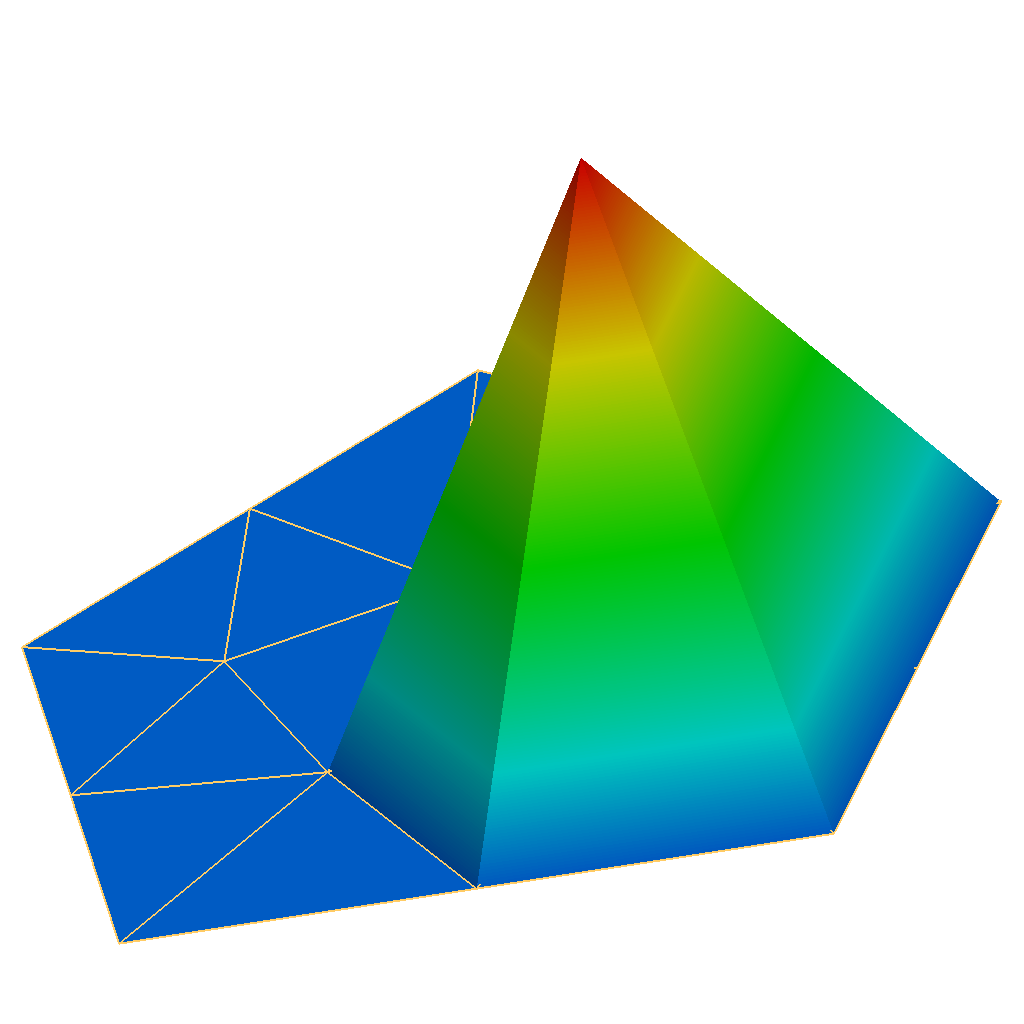
\includegraphics[width=0.49\textwidth]{p1_1}
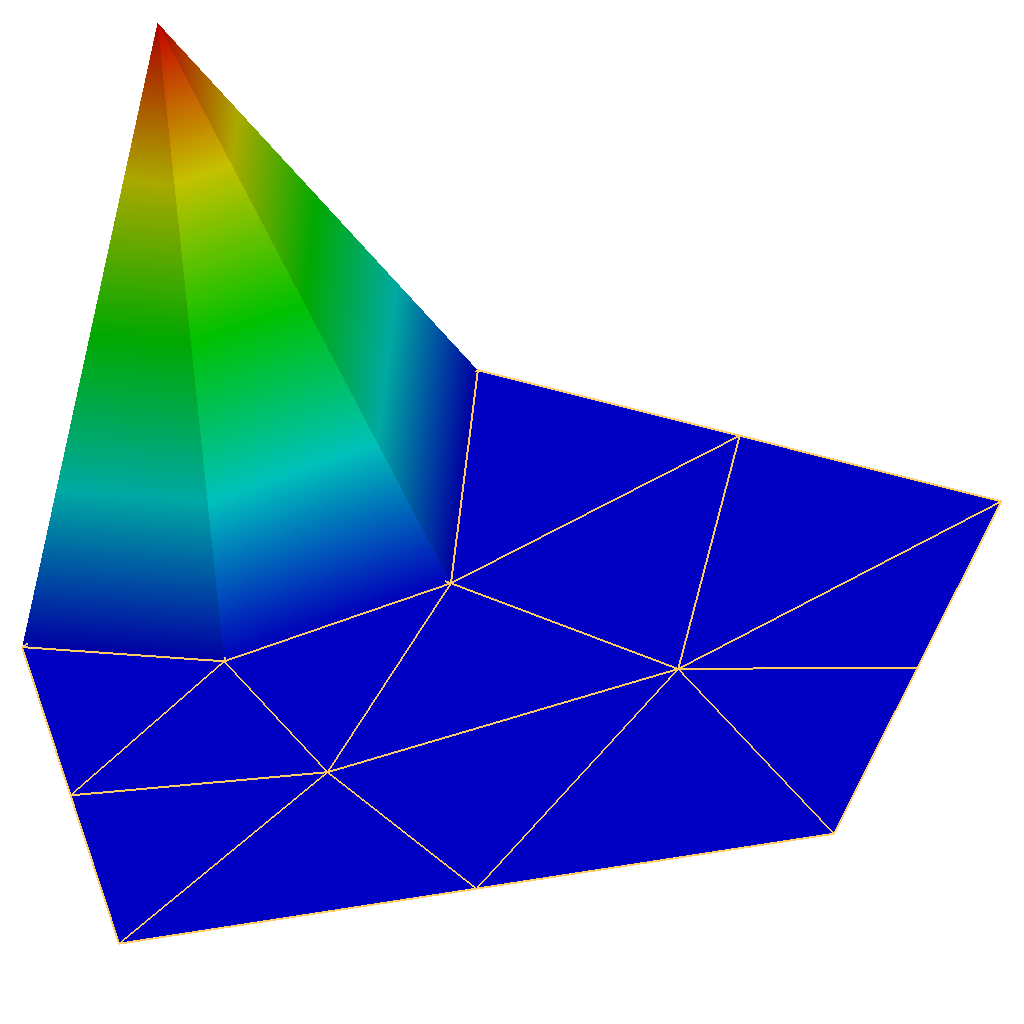
\includegraphics[width=0.49\textwidth]{p1_2}
\end{center}
Due to their shape they are often called {\em hat functions}
\end{frame}

\begin{frame}
\frametitle{Finite Element Solution}
Inserting a {\em basis representation} $u_h = \sum_{j=1}^N (z)_j \phi_j$ results in
\begin{align*}
a(u_h,v) &= l(v) \quad \forall v\in V_{h,0} &&\text{(discrete weak problem)},\nonumber \\
\Leftrightarrow
a\left(\sum_{j=1}^N (z)_j \phi_j,\phi_i\right) &= l(\phi_i) \quad \forall i\in \mathcal{I}_h^{int}
&&\text{(insert basis, linearity)}, \nonumber \\
\Leftrightarrow
\sum_{j=1}^N (z)_j a\left( \phi_j,\phi_i\right) &= l(\phi_i) \quad \forall i\in \mathcal{I}_h^{int}
&&\text{(linearity)}. \label{eq:linear1}
\end{align*}
Together with the condition $u_h\in V_{h,g}$ expressed as
\begin{equation*}
u_h(x_i) = z_i = g(x_i) \quad\forall i\in\mathcal{I}_h^{\partial\Omega}
\label{eq:linear2}
\end{equation*}
this forms a system of linear equations
$$Ax=b$$
where
\begin{equation*}
(A)_{i,j} = \left\{\begin{array}{ll}
a(\phi_j,\phi_i) & i\in\mathcal{I}_h^{int}\\
\delta_{i,j} & i\in\mathcal{I}_h^{\partial\Omega}
\end{array}\right., \quad
(b)_{i} = \left\{\begin{array}{ll}
l(\phi_i) & i\in\mathcal{I}_h^{int}\\
g(x_i) & i\in\mathcal{I}_h^{\partial\Omega}
\end{array}\right. .
\label{eq:systemdetail}
\end{equation*}
\end{frame}

\begin{frame}
\frametitle{Solution of Linear Systems}
\begin{itemize}
\item {\em Exact} solvers based on Gaussian elimination
\item This may become inefficent for {\em sparse} linear systems
\item {\em Iterative} methods (hopefully) produce a convergent sequence
$$\lim_{k\to\infty} z^k = z$$
\item A very simple example is {\em Richardson's} iteration:
$$ z^{k+1} = z^{k} + \omega (b-Az^{k})$$
requiring only {\em matrix-vector products}
\item Another well known class of iterative solvers are Krylov methods requiring
also only matrix-vector products
\end{itemize}
%\begin{algorithmic}
%\State Given $A, b, \epsilon$ and $z$ \Comment{input data}
%\State $d = b-Az$ \Comment{compute initial defect}
%\State $\tau = \epsilon \|d\|$ \Comment{compute target threshold}
%\While{$\|d\|\geq\tau$} \Comment{run until convergence}
%\State $z = z + \omega d$ \Comment{update solution}
%\State $y = A d$ \Comment{matrix-vector product}
%\State $d = d - \omega y$ \Comment{update defect}
%\EndWhile
%\end{algorithmic}
\end{frame}

\begin{frame}
\frametitle{Three Steps to Solve the FE Problem}
\begin{enumerate}
\item Assembling the matrix $A$. This mainly involves the computation of the matrix
elements $a(\phi_j,\phi_i)$ and storing them in an appropriate data structure.
\item Assembling the right hand side vector $b$. This mainly involves evaluations of
the right hand side functional $l(\phi_i)$.
\item {\em Alternatively:} Perform a matrix free operator evaluation $y=Az$. This involves evaluations
of $a(u_h,\phi_i)$ for all test functions $\phi_i$ and a given function $u_h$ due to:
\begin{align*}
(Az)_i &= \sum_{j=1}^N (A)_{i,j} (z)_j = \sum_{j=1}^N a(\phi_j,\phi_i) (z)_j \\
&= a\left(\sum_{j=1}^N (z)_j\phi_j,\phi_i\right) = a(u_h,\phi_i)
\end{align*}
\end{enumerate}
We now discuss {\em how} these steps may be implemented
\end{frame}

\begin{frame}
\frametitle{Four Important Tools}
\begin{enumerate}
\item Transformation formula for integrals. For $T\in\mathcal{T}_h$:
\begin{equation*}
\int_T y(x)\,dx = \int_{\hat T} y(\mu_T(\hat x)) |\det B_T| \,dx .
\end{equation*}
\item Midpoint rule on the reference element:
\begin{equation*}
\int_{\hat T} q(\hat x) \,dx \approx q(\hat S_d) w_d
\end{equation*}
(More accurate formulas are used later)
\item Basis functions via shape function transformation:
\begin{equation*}
\hat\phi_0(\hat x) = 1-\sum_{i=1}^d (\hat x)_i, \quad
\hat\phi_i(\hat x) = (\hat x)_i, i>0, \quad
\phi_{T,i}(\mu_T(\hat x)) = \hat\phi_i(\hat x)
\end{equation*}
\item Computation of gradients. For any $w(\mu_T(\hat x)) = \hat w(\hat x)$:
\begin{equation*}
B_T^T \nabla w(\mu_T(\hat x)) = \hat\nabla \hat w(\hat x) \quad\Leftrightarrow\quad
\nabla w(\mu_T(\hat x)) = B_T^{-T}\hat\nabla \hat w(\hat x) .
\end{equation*}
\end{enumerate}
\end{frame}

\begin{frame}
\frametitle{Assembly of Right Hand Side I}
In computing $(b)_i$ only the following elements are involved:
$$C(i) = \{(T,m)\in\mathcal{T}_h\times\{0,\ldots,d\} \,:\, g_T(m)=i\}$$
Then
\begin{align*}
(b)_i &= l(\phi_i) = \int_\Omega f \phi_i\,dx &&\text{(definition)} \\
&= \sum_{T\in\mathcal{T}_h} \int_T f \phi_i\,dx &&\text{(use mesh)} \\
&= \sum_{(T,m)\in C(i)} \int_{\hat T} f(\mu_T(\hat x)) \hat\phi_m(\hat x) |\det B_T|\,dx
&&\text{(localize)} \\
&= \sum_{(T,m)\in C(i)}
f(\mu_T(\hat S_d)) \hat\phi_m(\hat S_d) |\det B_T| w_d \, + \text{err}. &&\text{(quadrature)}
\end{align*}
\end{frame}

\begin{frame}
\frametitle{Assembly of Right Hand Side II}
\begin{itemize}
\item Now we need to perform these computations {\em for all $i\in\mathcal{I}_h^{int}$}!
\item Collect {\em element-local} computations:
\begin{equation*}
(b_T)_m =  f(\mu_T(\hat S_d)) \hat\phi_m(\hat S_d) |\det B_T| w_d \quad \forall m=0,\ldots,d
\end{equation*}
\item Define {restriction matrix} $R_T : \mathbb{R}^N \to \mathbb{R}^{d+1}$ with
\begin{equation*}
(R_T x)_m = (x)_i \quad \forall \,0\leq m \leq d, \,g_T(m)=i,
\end{equation*}
\item Then
\begin{equation*}
b = \sum_{T\in\mathcal{T}_h} R_T^T b_T .
\end{equation*}
\end{itemize}
\end{frame}

\begin{frame}
\frametitle{Assembly of Global Stiffness Matrix I}
In computing $(A)_{i,j}$ only the following elements are involved:
$$C(i,j) = \{(T,m,n)\in\mathcal{T}_h\times\{0,\ldots,d\} \,:\, g_T(m)=i \wedge g_T(n)=j\}$$
Then
{\small\begin{align*}
(A)_{i,j} &= a(\phi_j,\phi_i) = \int_\Omega \nabla \phi_j \cdot \nabla \phi_i \,dx
&&\text{(definition)}\\
&= \sum_{T\in\mathcal{T}_h} \int_T \nabla \phi_j \cdot \nabla \phi_i \,dx
&&\text{(use mesh)}\\
&= \sum_{(T,m,n)\in C(i,j)}
\int_{\hat T} (B_T^{-T} \hat\nabla\hat\phi_n(\hat x))\cdot (B_T^{-T} \hat\nabla\hat\phi_m(\hat x))
|\det B_T| \,d\hat x &&\text{(localize)}\\
&= \sum_{(T,m,n)\in C(i,j)}
(B_T^{-T} \hat\nabla\hat\phi_n(\hat S_d))\cdot (B_T^{-T} \hat\nabla\hat\phi_m(\hat S_d))
|\det B_T| w_d . &&\text{(quadrature)}
\end{align*}}
\end{frame}

\begin{frame}
\frametitle{Assembly of Global Stiffness Matrix II}
\begin{itemize}
\item Now we need to perform these computations for {\em  all} matrix entries!
\item Define the $d\times d+1$ matrix of shape function gradients
\begin{equation*}
\hat G = \left[\hat\nabla\hat\phi_0(\hat S_d)),\ldots,\hat\nabla\hat\phi_d(\hat S_d))\right] .
\end{equation*}
and the matrix of transformed gradients $$G=B_T^{-T} \hat G$$
\item Define the {\em local stiffness matrix}
\begin{equation*}
A_T = G^T G |\det B_T| w_d .
\end{equation*}
\item Then
\begin{equation*}
A =  \sum_{T\in\mathcal{T}_h} R_T^T A_T R_T .
\end{equation*}
\end{itemize}
\end{frame}

\begin{frame}
\frametitle{Matrix-free Operator Evaluation}
\begin{itemize}
\item Similar considerations apply for the operation $y=Az$
\item Pick out the coefficients on the element $T$:
$$z_T = R_T z$$
\item Perform the {\em element-local computation}:
\begin{equation*}
y_T = |\det B_T| w_d G^T G z_T
\end{equation*}
\item Accumulate the results:
\begin{equation*}
Az =  \sum_{T\in\mathcal{T}_h} R_T^T y_T.
\end{equation*}
\end{itemize}
\end{frame}

\begin{frame}
\frametitle{Implementation Summary}
\begin{itemize}
\item All necessary steps in the solution procedure have the following general form:
\begin{algorithmic}[1]
\For{$T\in\mathcal{T}_h$} \Comment{loop over mesh elements}
\State $z_T = R_T z$ \Comment{load element data}
\State $q_T=\text{compute}(T,z_T)$ \Comment{element local computations}
\State $\text{Accumulate}(q_T)$ \Comment{store result in global data structure}
\EndFor
\end{algorithmic}
\item PDELab provides a generic {\em assembler} that performs all these steps,
except (3) which needs to be supplied by the implementor of a FEM
\item All these concepts carry over to
\begin{itemize}
\item Nonlinear problems
\item Time-dependent problems
\item Systems of PDEs
\item High-order methods
\item Other schemes such as FVM, nonconforming FEM
\item Parallel computations
\end{itemize}
\end{itemize}
\end{frame}

\begin{frame}
\frametitle{Residual Forms}
\begin{itemize}
\item The FEM based on the weak formulation formulation may equivalently
be written as
\begin{equation*}
\text{Find $u_h\in U_h$ s.t.:} \quad r_h^\text{Poisson}(u_h,v)=0 \quad \forall v\in V_h.
\end{equation*}
where $r^\text{Poisson}(u_h,v) = a(u_h,v) - l(v)$ is the \textbf{residual form}
\item This residual form is {\em affine linear} in $u_h$ and {\em linear} in $v$
\item A {\em nonlinear} PDE results in a residual form $r(u,v)$ that is {\em nonlinear}
in its first argument
\item Residual forms are always linear in the second argument due
to linearity of the integral
\item \textbf{PDELab uses the concept of a residual form as its main abstraction!}
\end{itemize}
\end{frame}

\begin{frame}
\frametitle{Generalization}
\begin{itemize}
\item More complicated discretization schemes:
\begin{equation*}
\begin{split}
r(u,v) &=
\sum_{T\in\mathcal{T}_h} \alpha_T^V(R_T u, R_T v)
+ \sum_{T\in\mathcal{T}_h} \lambda_T^V(R_T v) \\
&\qquad+ \sum_{F\in\mathcal{F}_h^i} \alpha_F^S(R_{T_F^-} u,R_{T_F^+} u, R_{T_F^-} v, R_{T_F^+} v)\\
&\qquad+ \sum_{F\in\mathcal{F}_h^{\partial\Omega}} \alpha_F^B(R_{T_F^-} u, R_{T_F^-} v)
+ \sum_{F\in\mathcal{F}_h^{\partial\Omega}} \lambda_F^B(R_{T_F^-} v) .
\end{split}
\end{equation*}
\item Instationary problems: Find $u_h(t)\in U_h$ s.t.:
\begin{equation*}
d_t m_h(u_h(t),v;t) + r_h(u_h(t),v;t) = 0
\quad \forall v\in V_h
\end{equation*}
\item Systems of PDEs: Find $u_h\in U_h=U_h^1\times \ldots \times U_h^s$ s.t.:
\begin{equation*}
r_h(u_h,v)=0
\quad \forall v\in V_h=V_h^1\times\ldots\times V_h^s
\end{equation*}
\end{itemize}
\end{frame}


\begin{frame}
\begin{center}
\Large\textbf{Implementation in DUNE/PDELab}
\end{center}
\end{frame}

\begin{frame}
\frametitle{The Duniverse}
\begin{center}
\small
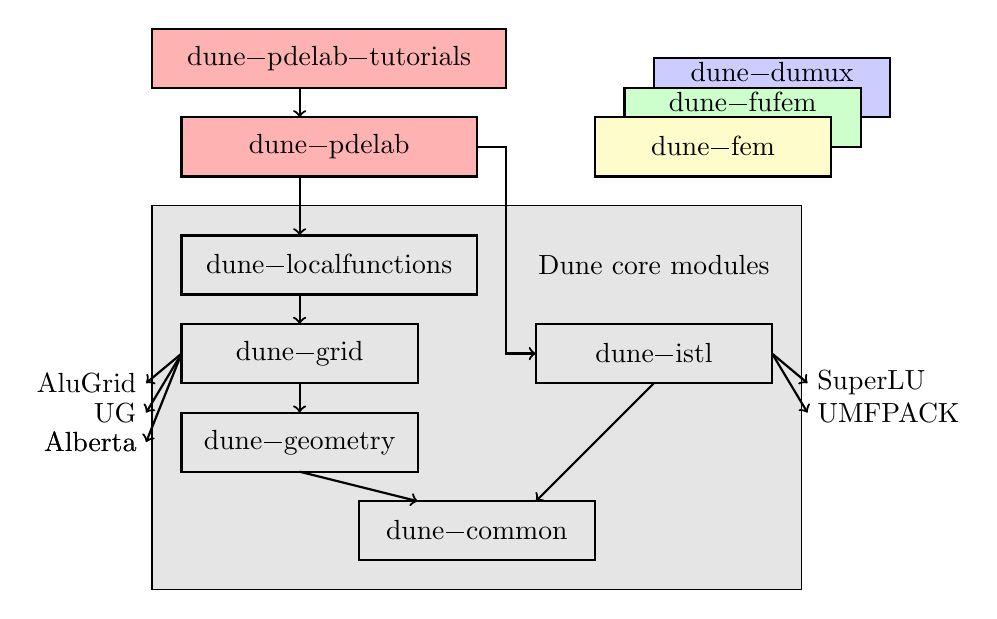
\begin{tikzpicture}[scale=0.75]
\filldraw[thin,fill=black!10!white] (1.5,-0.5)  rectangle (12.5,6);
\draw[thick] (5,0)  rectangle (9,1);
\node at (7,0.5) {\lstinline{dune-common}};
\draw[thick] (2,1.5)  rectangle (6,2.5);
\node at (4,2) {\lstinline{dune-geometry}};
\draw[thick,->] (4,1.5) -- (6,1);
\draw[thick] (2,3)  rectangle (6,4);
\node at (4,3.5) {\lstinline{dune-grid}};
\draw[thick,->] (4,3) -- (4,2.5);
\draw[thick] (8,3)  rectangle (12,4);
\node at (10,3.5) {\lstinline{dune-istl}};
\draw[thick,->] (10,3) -- (8,1);
\draw[thick] (2,4.5)  rectangle (7,5.5);
\node at (4.5,5) {\lstinline{dune-localfunctions}};
\draw[thick,->] (4,4.5) -- (4,4);
\node at (10,5) {Dune core modules};
\filldraw[thick,fill=red!30!white] (2,6.5)  rectangle (7,7.5);
\node at (4.5,7) {\lstinline{dune-pdelab}};
\filldraw[thick,fill=red!30!white] (1.5,8)  rectangle (7.5,9);
\node at (4.5,8.5) {\lstinline{dune-pdelab-tutorials}};
\draw[thick,->] (4,6.5) -- (4,5.5);
\draw[thick,->] (4,8) -- (4,7.5);
\draw[thick,->] (7,7) -- (7.5,7) -- (7.5,3.5) -- (8,3.5);
\filldraw[thick,fill=blue!20!white] (10,7.5)  rectangle (14,8.5);
\node at (12,8.25) {\lstinline{dune-dumux}};
\filldraw[thick,fill=green!20!white] (9.5,7)  rectangle (13.5,8);
\node at (11.5,7.75) {\lstinline{dune-fufem}};
\filldraw[thick,fill=yellow!20!white] (9,6.5)  rectangle (13,7.5);
\node at (11,7) {\lstinline{dune-fem}};
\node[right] at (12.6,3) {SuperLU};
\node[right] at (12.6,2.5) {UMFPACK};
\draw[thick,->] (12,3.5) -- (12.6,3);
\draw[thick,->] (12,3.5) -- (12.6,2.5);
\node[left] at (1.4,3) {AluGrid};
\node[left] at (1.4,2.5) {UG};
\node[left] at (1.4,2.0) {Alberta};
\node[left] at (1.4,2.0) {Alberta};
\draw[thick,->] (2,3.5) -- (1.4,3);
\draw[thick,->] (2,3.5) -- (1.4,2.5);
\draw[thick,->] (2,3.5) -- (1.4,2);
\end{tikzpicture}
\end{center}
\end{frame}

\begin{frame}
\frametitle{The PDE Problem Revisited}
We solve Poisson's equation with inhomogeneous Dirichlet boundary conditions:
\begin{align*}
-\Delta u & = f \qquad\text{in $\Omega$}\\
u &= g \qquad\text{on $\partial\Omega$}
\end{align*}
The weak formulation is
\begin{equation*}
u \in V_g :\qquad a(u,v) = l(v) \qquad \forall v\in V_0
\end{equation*}
with
$$a(u,v) = \int_\Omega \nabla u \cdot \nabla v \,dx  \quad\text{and}\quad
l(v)=\int_\Omega fv\, dx $$
and
\begin{align*}
V_0 &= H_0^1(\Omega) \\
V_g &= \{ v\in H^1(\Omega) \,:\, v = u_g + w \wedge u_g|\Gamma_D=g \wedge w\in V_0 \}
\end{align*}
\end{frame}

\begin{frame}
\frametitle{Generic Assembly Loop}
\begin{algorithmic}[1]
\For{$T\in\mathcal{T}_h$} \Comment{loop over mesh elements}
\State $z_T = R_T z$ \Comment{load element data}
\State $q_T=\text{compute}(T,z_T)$ \Comment{element local computations}
\State $\text{Accumulate}(q_T)$ \Comment{store result in global data structure}
\EndFor
\end{algorithmic}
Only the computational kernels $\text{compute}(T,z_T)$ need to be implemented by the user
to implement the finite element method
\end{frame}

\begin{frame}
\frametitle{Assembly of Right Hand Side}
\begin{itemize}
\item Now we need to perform these computations {\em for all $i\in\mathcal{I}_h^{int}$}!
\item Collect {\em element-local} computations:
\begin{equation*}
(b_T)_m =  f(\mu_T(\hat S_d)) \hat\phi_m(\hat S_d) |\det B_T| w_d \quad \forall m=0,\ldots,d
\end{equation*}
\item Define {destriction matrix} $R_T : \mathbb{R}^N \to \mathbb{R}^{d+1}$ with
\begin{equation*}
(R_T x)_m = (x)_i \quad \forall \,0\leq m \leq d, \,g_T(m)=i,
\end{equation*}
\item Then
\begin{equation*}
b = \sum_{T\in\mathcal{T}_h} R_T^T b_T .
\end{equation*}
\end{itemize}
\end{frame}

\begin{frame}
\frametitle{Assembly of Global Stiffness Matrix}
\begin{itemize}
\item Define the $d\times d+1$ matrix of shape function gradients
\begin{equation*}
\hat G = \left[\hat\nabla\hat\phi_0(\hat S_d)),\ldots,\hat\nabla\hat\phi_d(\hat S_d))\right] .
\end{equation*}
and the matrix of transformed gradients $$G=B_T^{-T} \hat G$$
\item Define the {\em local stiffness matrix}
\begin{equation*}
A_T = G^T G |\det B_T| w_d .
\end{equation*}
\item Then
\begin{equation*}
A =  \sum_{T\in\mathcal{T}_h} R_T^T A_T R_T .
\end{equation*}
\end{itemize}
\end{frame}

\begin{frame}
\frametitle{Matrix-free Operator Evaluation}
\begin{itemize}
\item Similar considerations apply for the operation $y=Az$
\item Pick out the coefficients on the element $T$:
$$z_T = R_T z$$
\item Perform the {\em element-local computation}:
\begin{equation*}
y_T = |\det B_T| w_d G^T G z_T
\end{equation*}
\item Accumulate the results:
\begin{equation*}
Az =  \sum_{T\in\mathcal{T}_h} R_T^T y_T.
\end{equation*}
\end{itemize}
\end{frame}

\begin{frame}
\frametitle{Overview DUNE/PDELab Implementation}
Files involved are:
\begin{enumerate}[1)]
\item File \lstinline{tutorial00.cc}
\begin{itemize}
\item Includes C++, DUNE and PDELab header files
\item Includes all the other files
\item Contains the \lstinline{main} function
\item Creates a finite element mesh and calls the \lstinline{driver}
\end{itemize}
\item File \lstinline{tutorial00.ini}
\begin{itemize}
\item Contains parameters controlling the execution
\end{itemize}
\item File \lstinline{driver.hh}
\begin{itemize}
\item Function \lstinline{driver} setting up and solving the finite element problem
\end{itemize}
\item File \lstinline{poissonp1.hh}
\begin{itemize}
\item Class \lstinline{PoissonP1}
realizing the necessary element-local computations
\end{itemize}
\end{enumerate}
Now lets go to the code \ldots
\end{frame}

\end{document}
